\documentclass[border=7pt]{standalone}
\usepackage{tikz}
\usetikzlibrary{decorations.pathreplacing}

\begin{document}
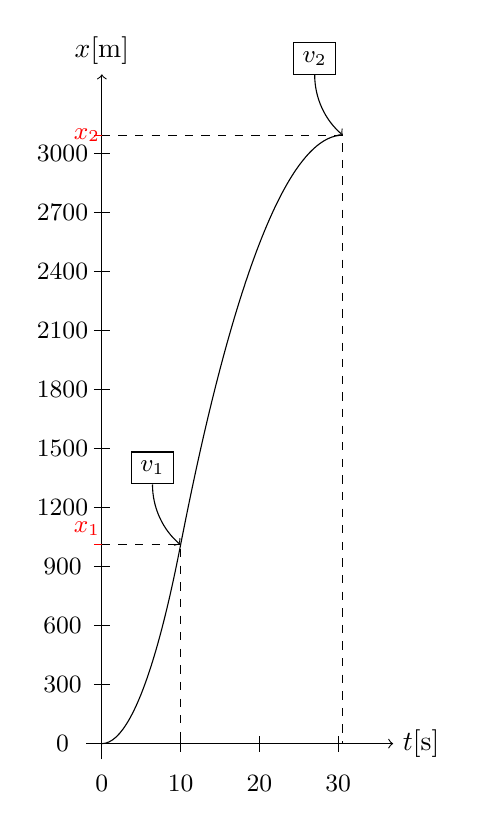
\begin{tikzpicture}
  \draw [->] (-0.2,0) -- (3.7,0)node[anchor=west]{$t$[s]};
  \draw [->] (0,-0.2) -- (0,8.5)node[anchor=south]{$x$[m]};
  \foreach \x in {0,10,...,30}{
    \draw (\x/10,-0.5) node{\small\x};
    \draw (\x/10,-0.1) -- (\x/10,0.1);
    };
  \foreach \x in {0,300,...,3000}{
    \draw (-0.5,\x/400) node{\small\x};
    \draw (-0.1,\x/400) -- (0.1,\x/400);
    };
  \draw [red](-0.1,1010/400) -- (0.1,1010/400) node[anchor=south east]{\small $x_1$};
  \draw [red](-0.1,3091/400) -- (0.1,3091/400) node[anchor=east]{\small $x_2$};

  \draw [dashed] (0, 1010/400) -- (10/10,1010/400) -- (10/10,0);
  \draw [dashed] (0,3091/400) -- (30.6/10,3091/400)--(30.6/10, 0);

  \draw [<-](10/10,1010/400) arc(230:180:1)node [anchor= south, draw,align=center, fill=white] {\small $v_1$};
  \draw [<-](3.06,3091/400) arc(230:180:1)node [anchor= south, draw,align=center, fill=white] {\small $v_2$};
  %\draw [<-](5.56,0) arc(230:180:1)node [anchor= south, draw,align=center, fill=white] {\small $v_3$};

  %\draw [blue,decorate,decoration={brace,amplitude=6pt}] (0,0) -- (1,0) node [black,midway, yshift=0.4 cm] {$t_1$} ;
  %\draw [blue,decorate,decoration={brace,amplitude=6pt}] (1,0) -- (3.06,0) node [black,midway, yshift=0.4 cm] {$t_2$} ;
  %\draw [blue,decorate,decoration={brace,amplitude=6pt}] (3.06,0) -- (5.56,0) node [black,midway, yshift=0.4 cm] {$t_3$} ;


  %\draw [red](10/10,-0.1) -- (10/10,0.1)node[anchor=south west]{$t_1$};
  %\draw [red](30.6/10,-0.1) -- (30.6/10,0.1) node[anchor=south west ]{$t_1+t_2$};
  %\draw [red](5.56,-0.1) -- (5.56,0.1) node[anchor=south west ]{$t_1+t_2+t_3$};

  \draw (0,0) parabola  (1,1010/400);
  \draw (1,1010/400) parabola [bend at end](3.06,3091/400);
  %\draw (3.06,3091/400)  parabola [bend at start] (5.56,0);



\end{tikzpicture}
\end{document}
